\section{Experimental Results}
\label{sec:experiment}
In this section, we discuss the experimental setup of the implementation evaluation.
We demonstrate how the experiments were performed step-by-step by solving problems
that we faced during implementation.
We state the latency and accuracy of the implemented parallel shortest path algorithm based on
Dijkstra's single pair shortest path algorithm for different clustering techniques and
configurations. For each of the experiments, we run 10 times by randomly picking source and
destination nodes for the shortest path. Each time we run for all types of clustering configurations
for fair comparison of accuracy and latency.

\subsection{Experimental Setup}
\label{sec:setup}
\subsubsection{Testbed}
We run the experiments on \textit{Innovation}, an HPC cluster maintained by the Computer Architecture
and Systems Research Laboratory (CASTL)~\cite{castl}. In this cluster, each node has 10 dual-socket
Intel Xeon(R) CPU E5-2650 cores, 64 GB memory, and a 1 TB Seagate ST91000640NS SATA disk.
The communication network is build on FDR InfiniBand interconnect with Mellanox ConnectX-5 NIC.
\subsubsection{Configurations}
In the experiments, we have used MPICH-3.1 as the communication substrate for running in the distributed
environment. We follow a data parallel approach where each clustered graph is assigned to each
client in the system. We choose the total number of processes equal to the number of clients, so
that each client is assigned exactly one process.

\subsection{Evaluation}
\label{sec:eval}
In this section, we discuss the latency breakdown on different phases of the implementation process
followed by accuracy measurement. We use MPI.Wtime for logging the time of each part of the total execution
time. For each of the clustering techniques, we compare the output, i.e., final shortest path, with the path
determined from the experiments on clustering with k=1 where the whole graph data is fed to the system.
We demonstrate these two metrics by increasing the number of clusters from 1 to 8 in geometric order for
both K-means and Agglomerative clustering. We dumped pickle files for each cluster when we preprocessed the
whole graph representation of the map of Tallahassee offline using \texttt{prepare\_cluster.py} file.
As shown in \figurename~\ref{fig:init_eval}, in the intial stage implementation, we run the experiments
for both K-means and Agglomerative clustering. We analyze the latency breakdown to pinpoint the exact
cause of the performance overhead and found that the main bottleneck was in the user space instead of
being in the kernel space for communication due to the distributed architecture. So, we improved the
algorithm and ran all the experiments again for all clustering configurations as demonstrated in
\figurename~\ref{fig:impr_eval}

\begin{figure*}[h!]
    \vspace{-0.0pc}
    \begin{center}
       \subfigure[Latency (K-means)\label{fig:kmeans_init_latency}]
       {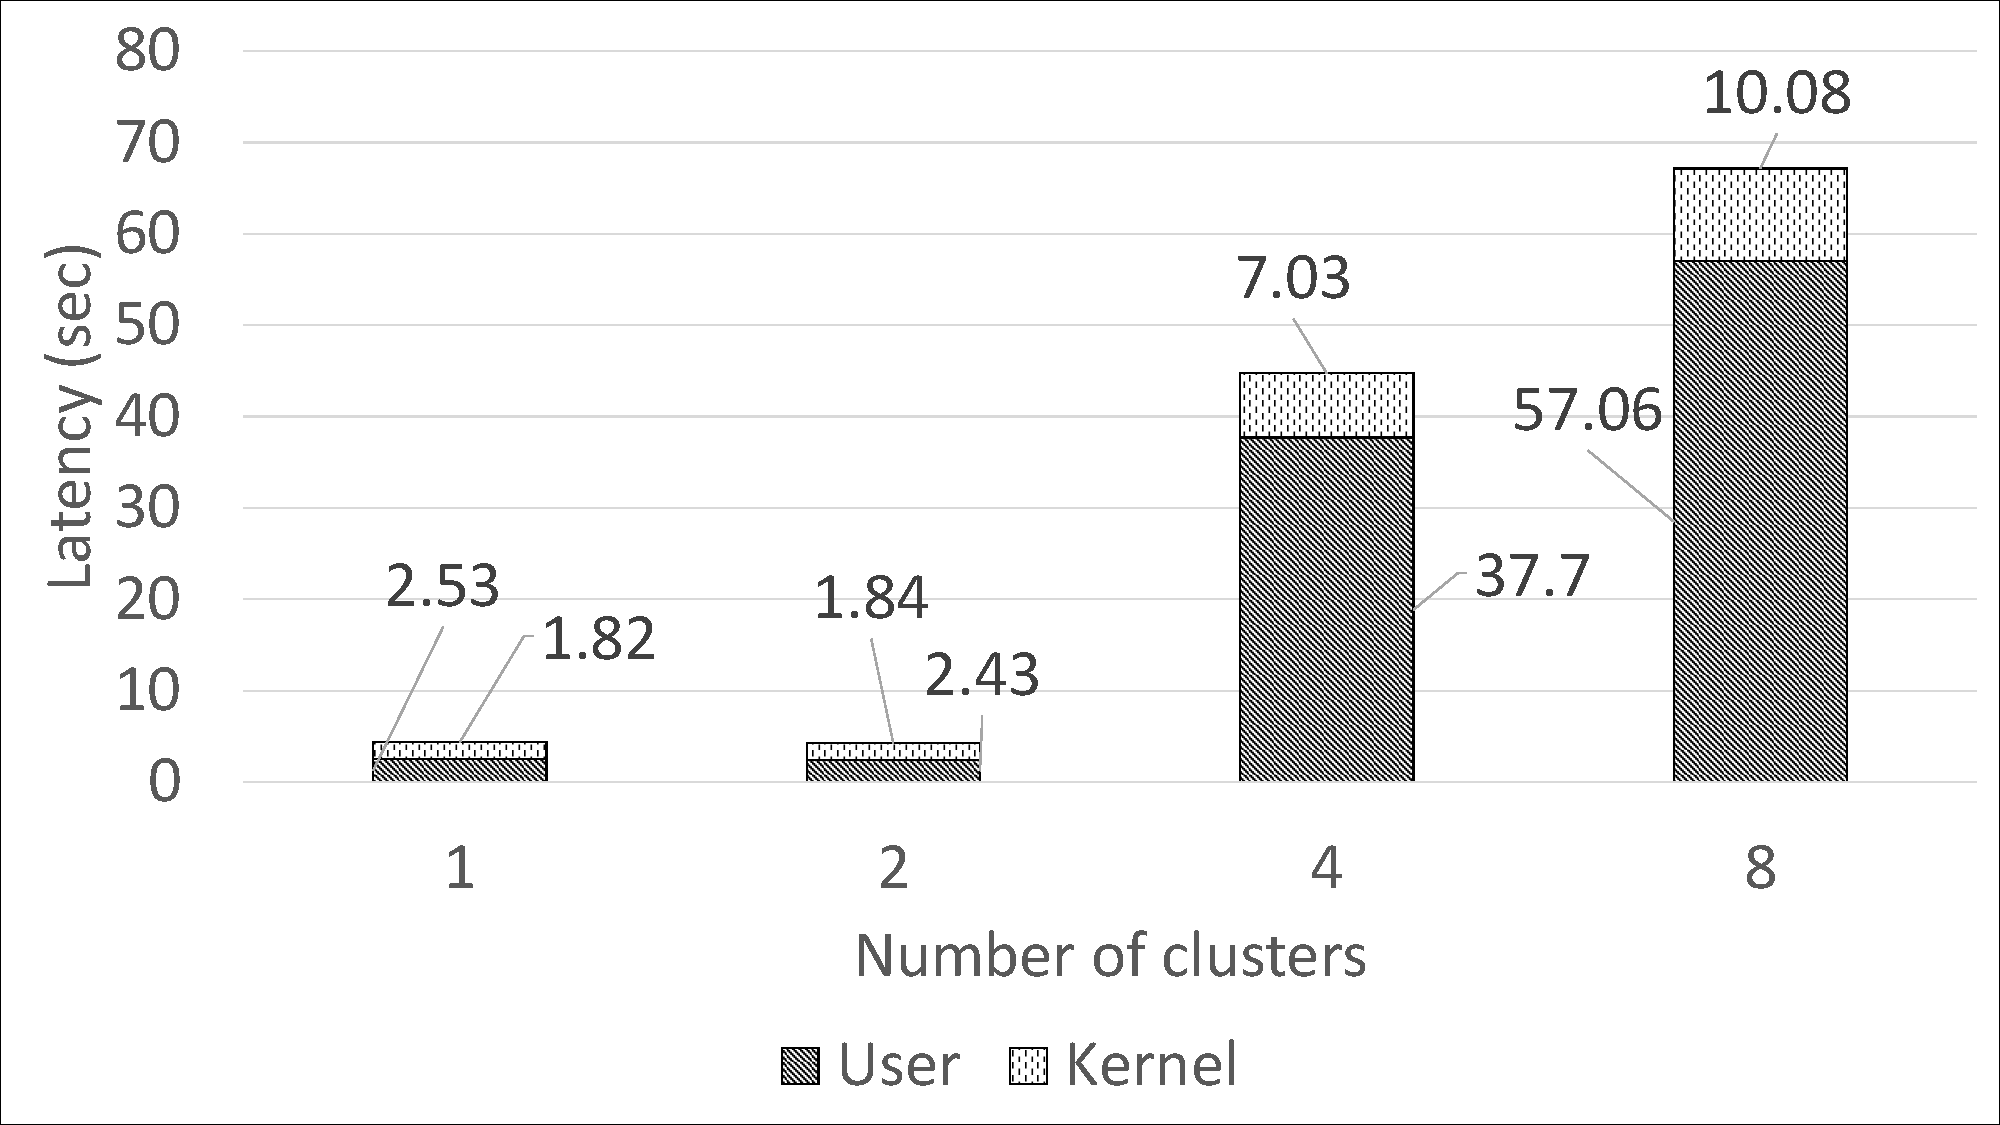
\includegraphics[width=0.4\textwidth]{evaluation/kmeans_latency_initial.pdf}}
       \subfigure[Latency (Agglomerative)\label{fig:agglomerative_init_latency}]
       {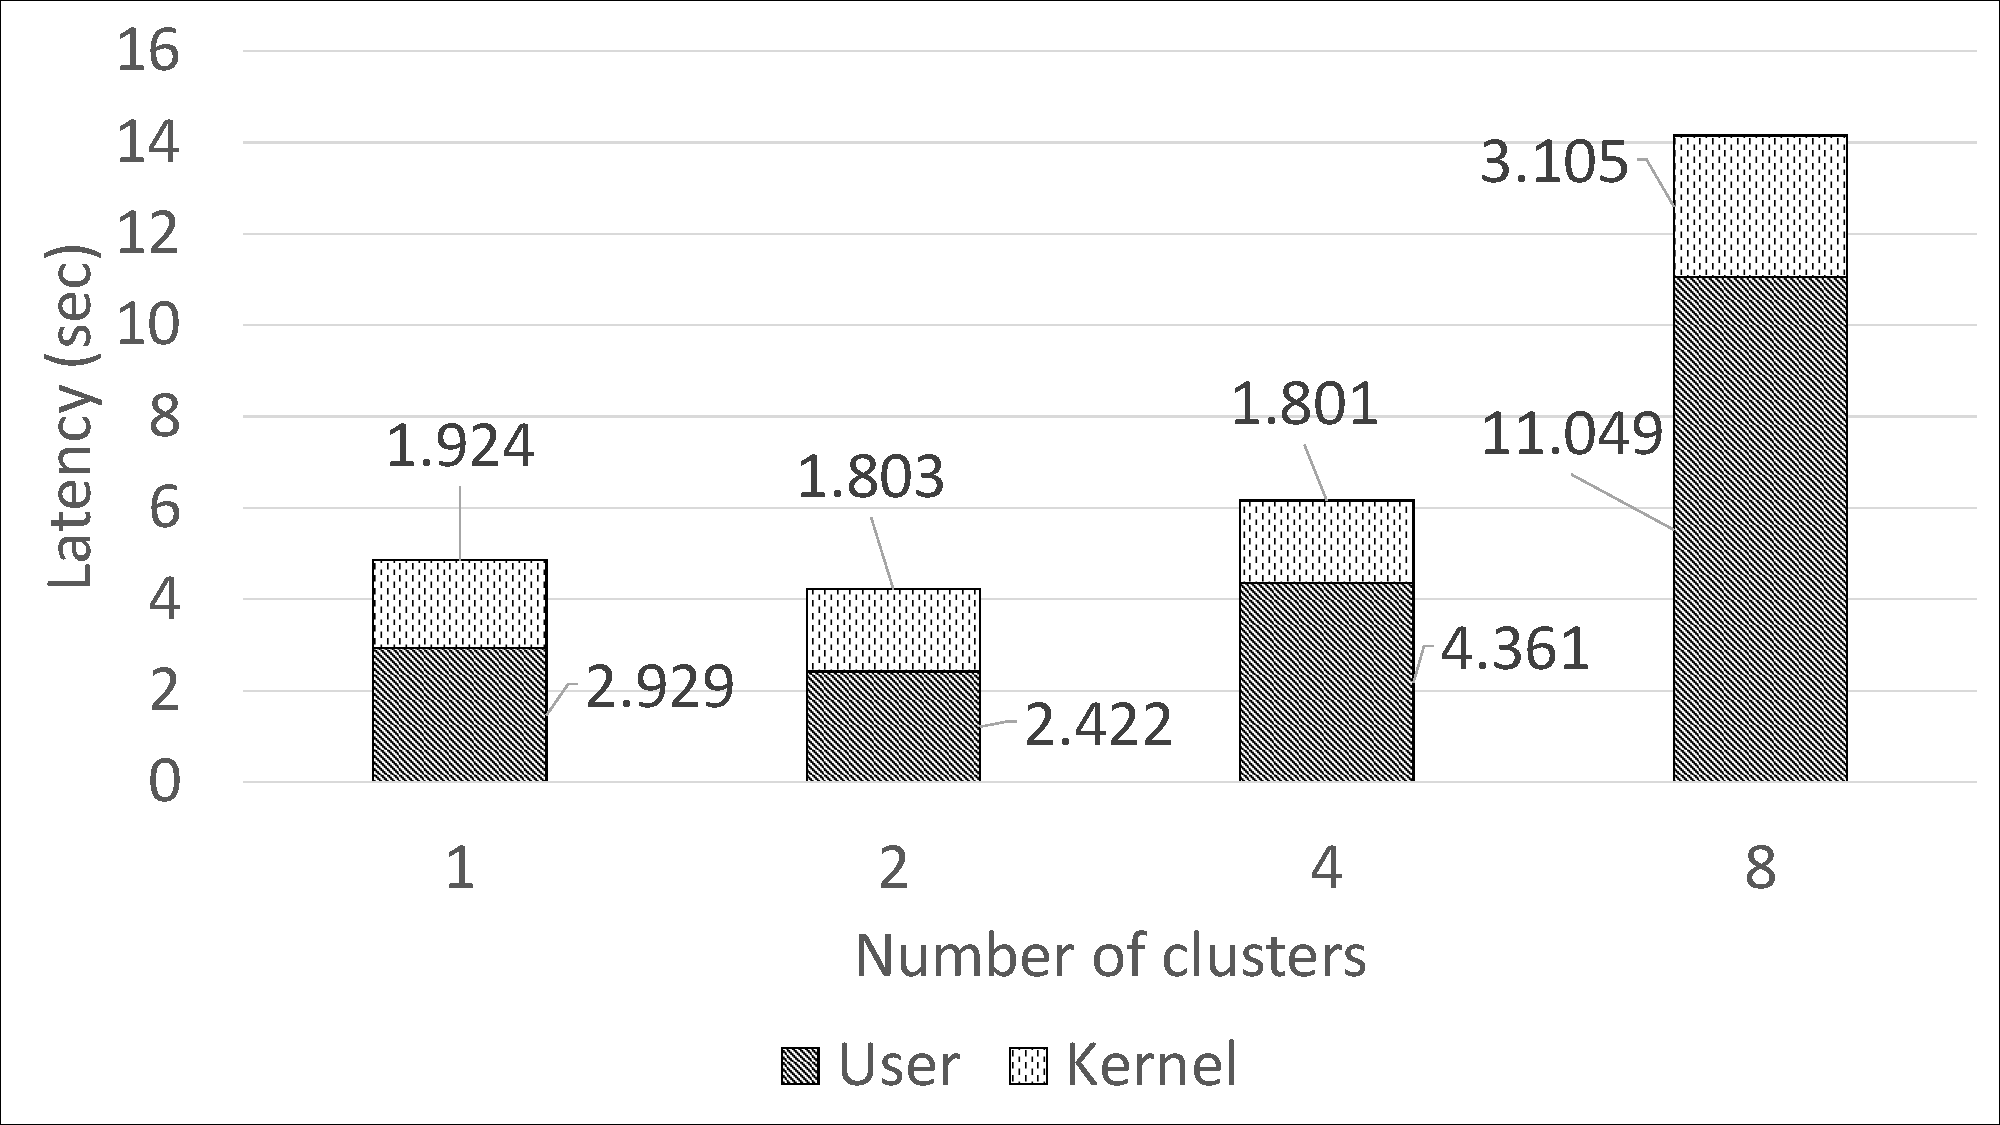
\includegraphics[width=0.4\textwidth]{evaluation/agglomerative_latency_initial.pdf}}
       \subfigure[Accuracy (K-means)\label{fig:kmeans_init_accuracy}]
       {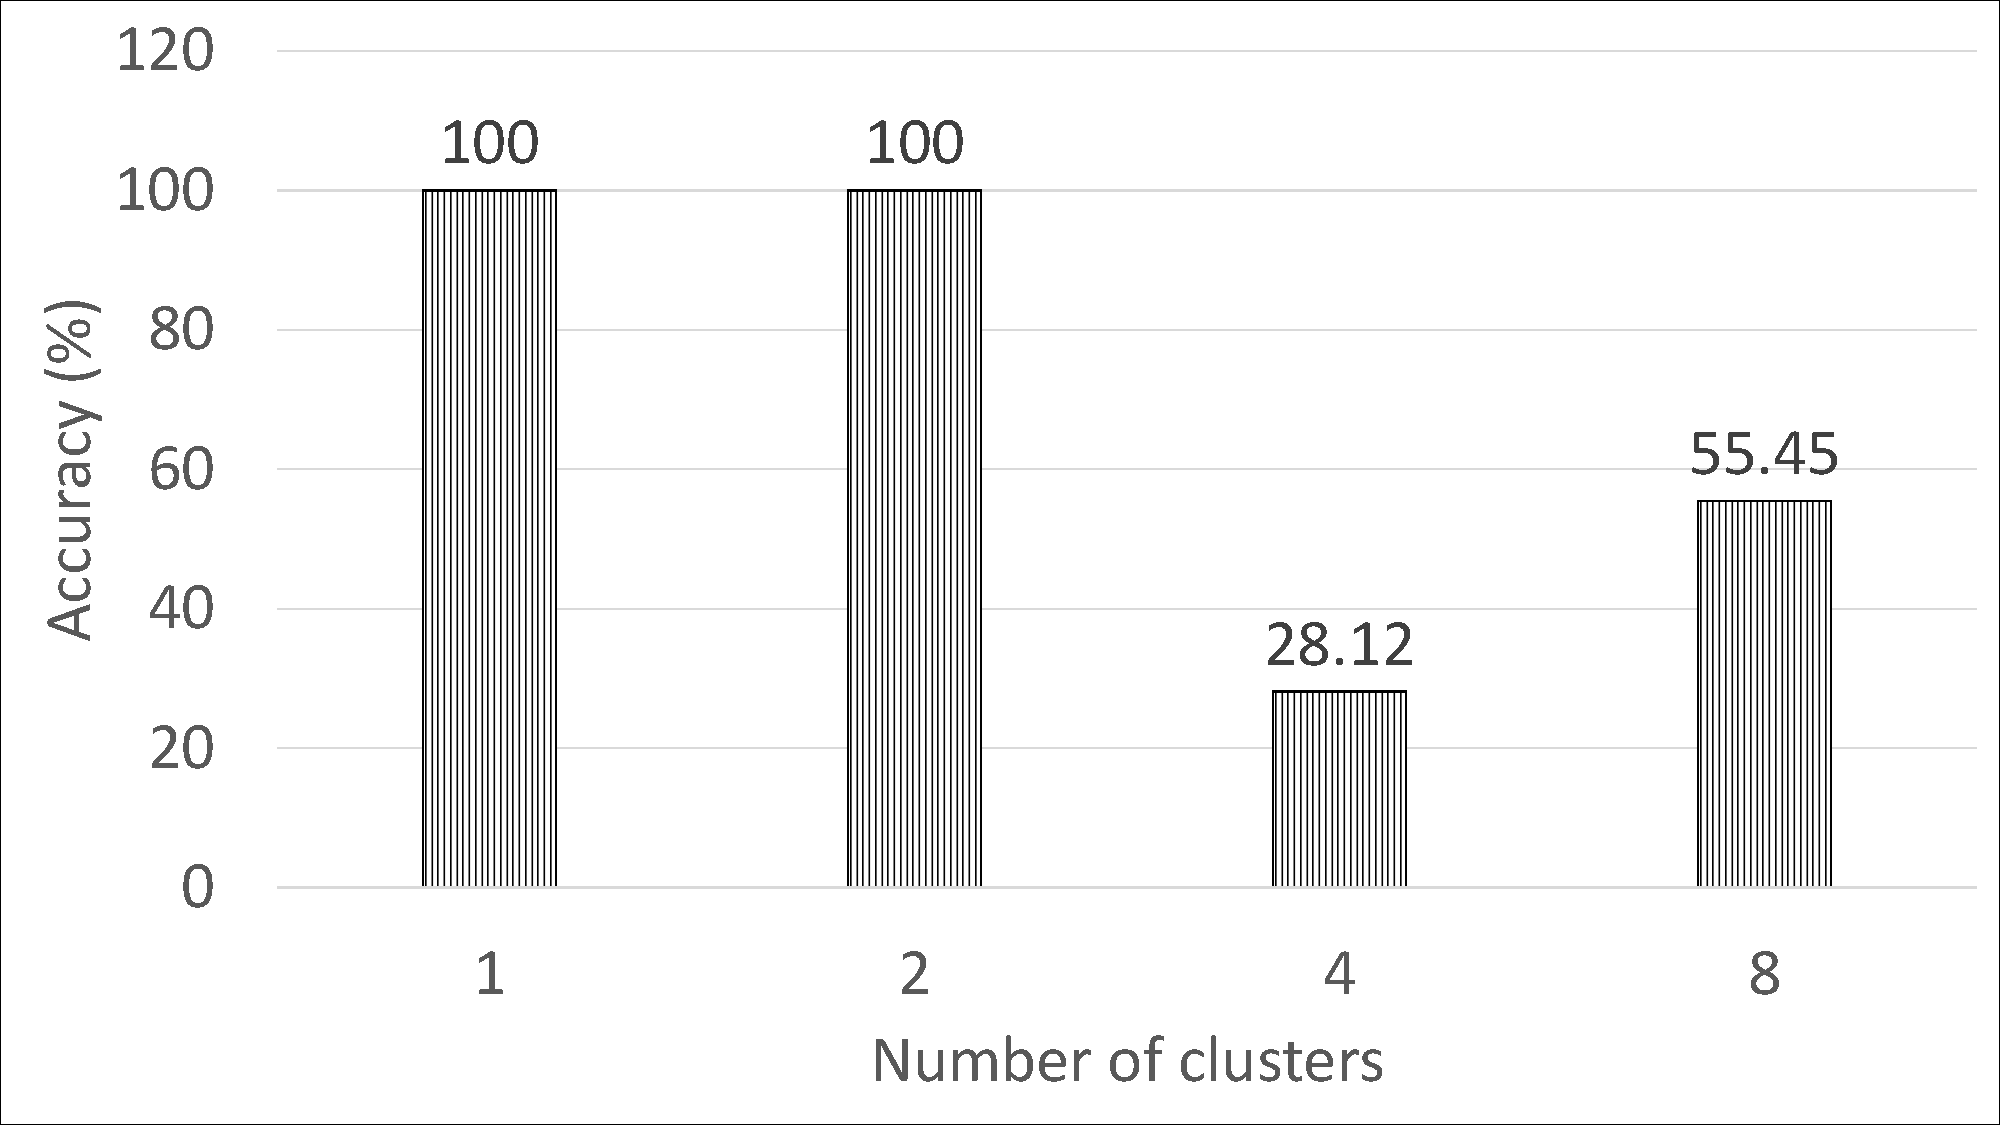
\includegraphics[width=0.4\textwidth]{evaluation/kmeans_accuracy_initial.pdf}}
       \subfigure[Accuracy (Agglomerative)\label{fig:agglomerative_init_accuracy}]
       {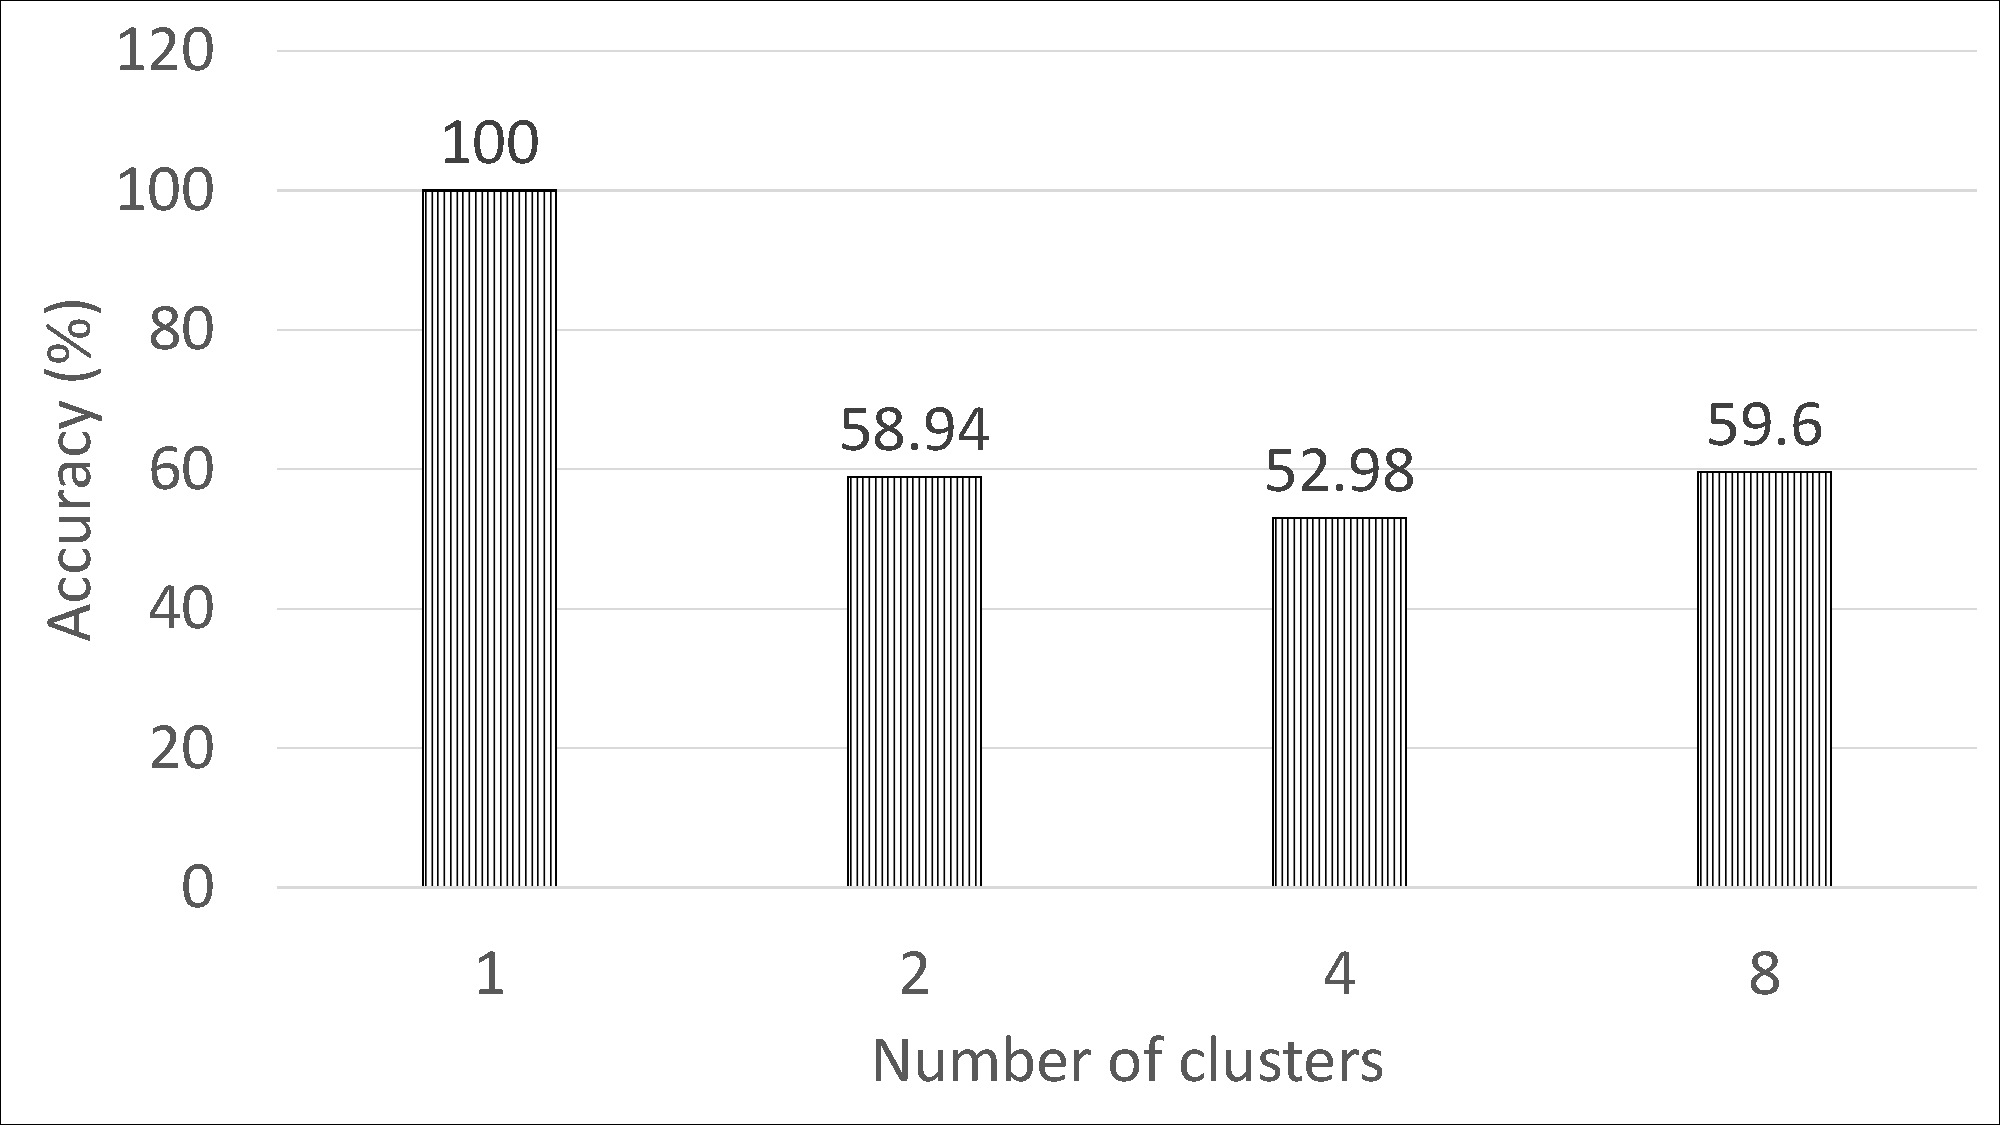
\includegraphics[width=0.4\textwidth]{evaluation/agglomerative_accuracy_initial.pdf}}
       \vspace{-0.0pc}
       \caption{Initial latency breakdown and accuracy for distributed shortest path detection algorithm on data clustered using K-means and Agglomerative clustering}
       \label{fig:init_eval}
    \end{center}
  \vspace{-1.0pc}
\end{figure*}

\begin{figure*}[h!]
    \vspace{-0.0pc}
    \begin{center}
        \subfigure[Latency (K-means)\label{fig:kmeans_impr_latency}]
        {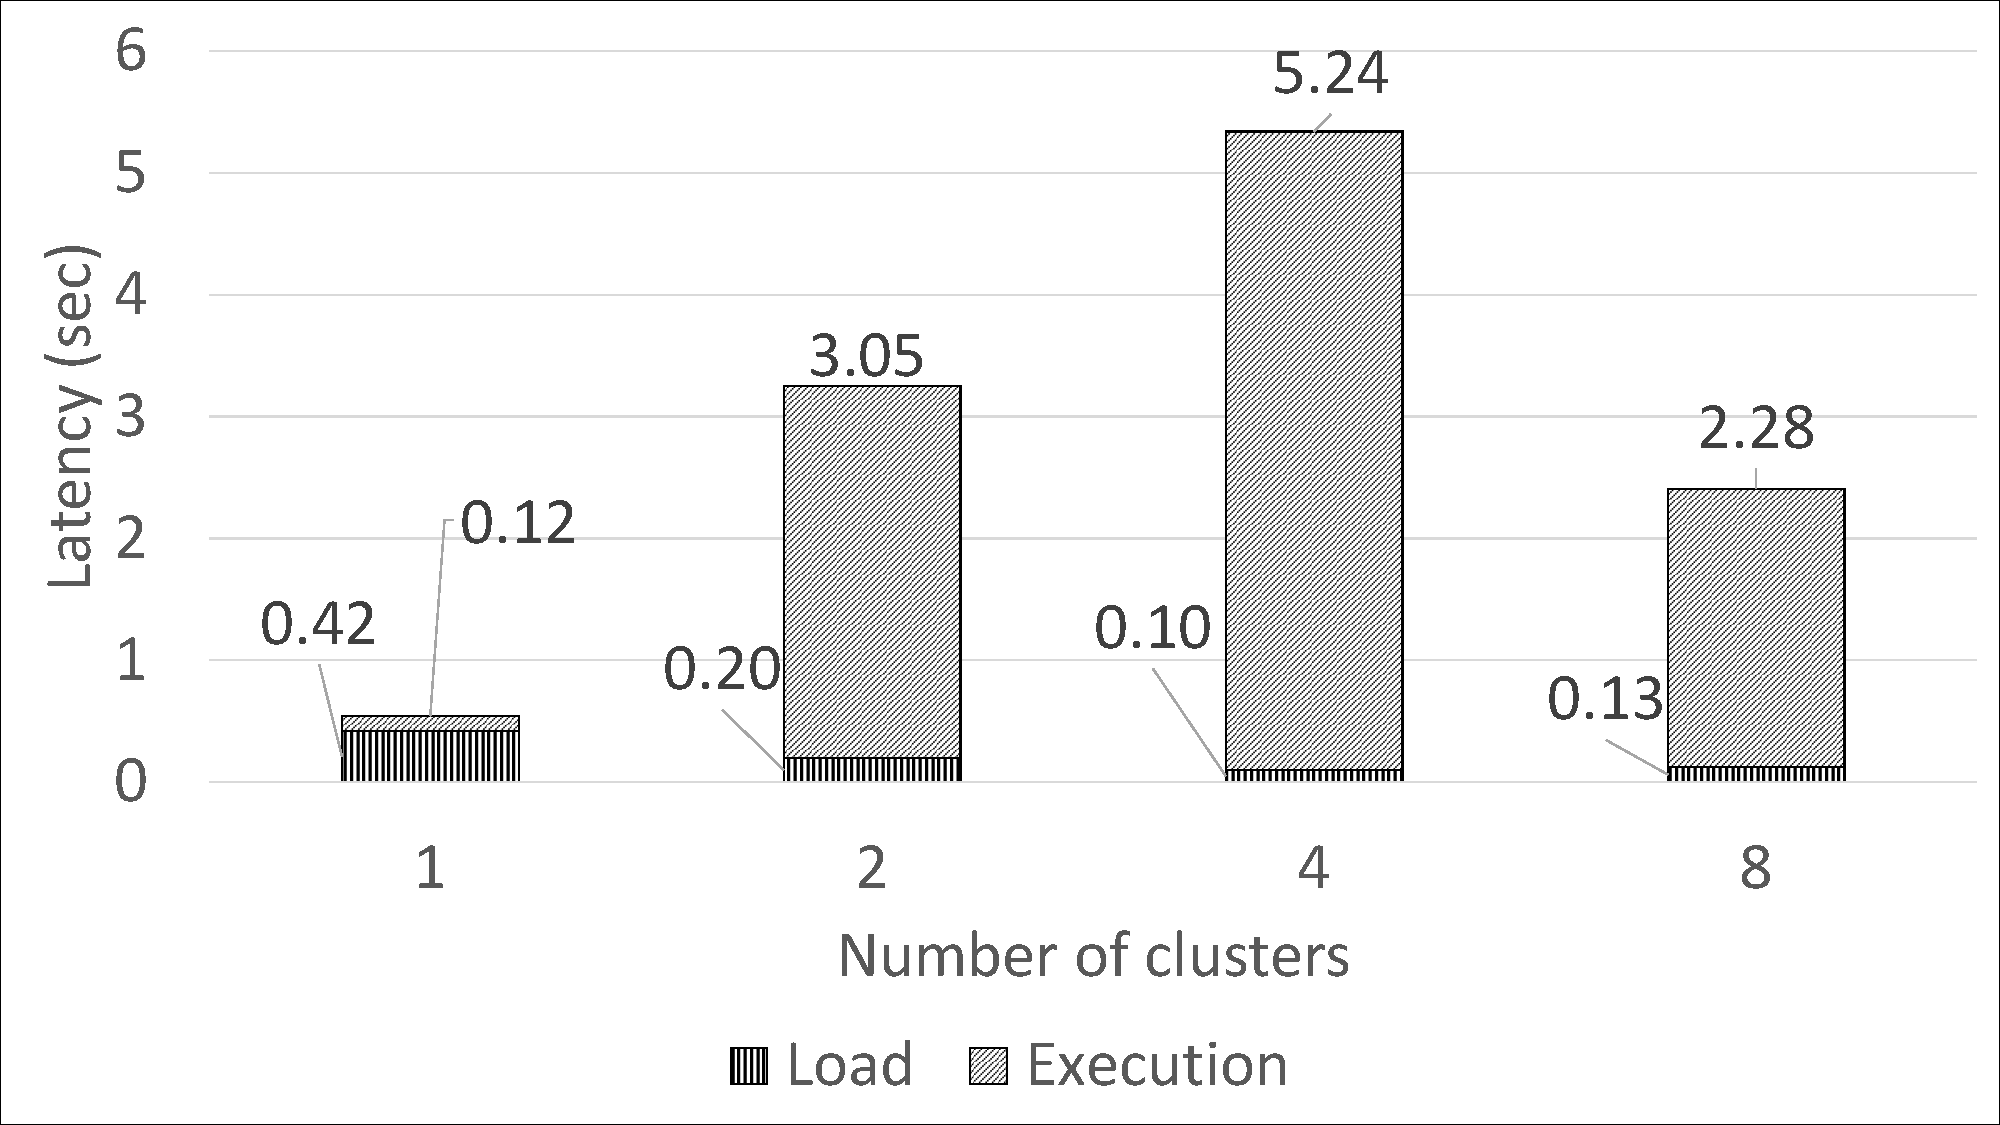
\includegraphics[width=0.4\textwidth]{evaluation/kmeans_latency.pdf}}
       \subfigure[Latency (Agglomerative)\label{fig:agglomerative_impr_latency}]
       {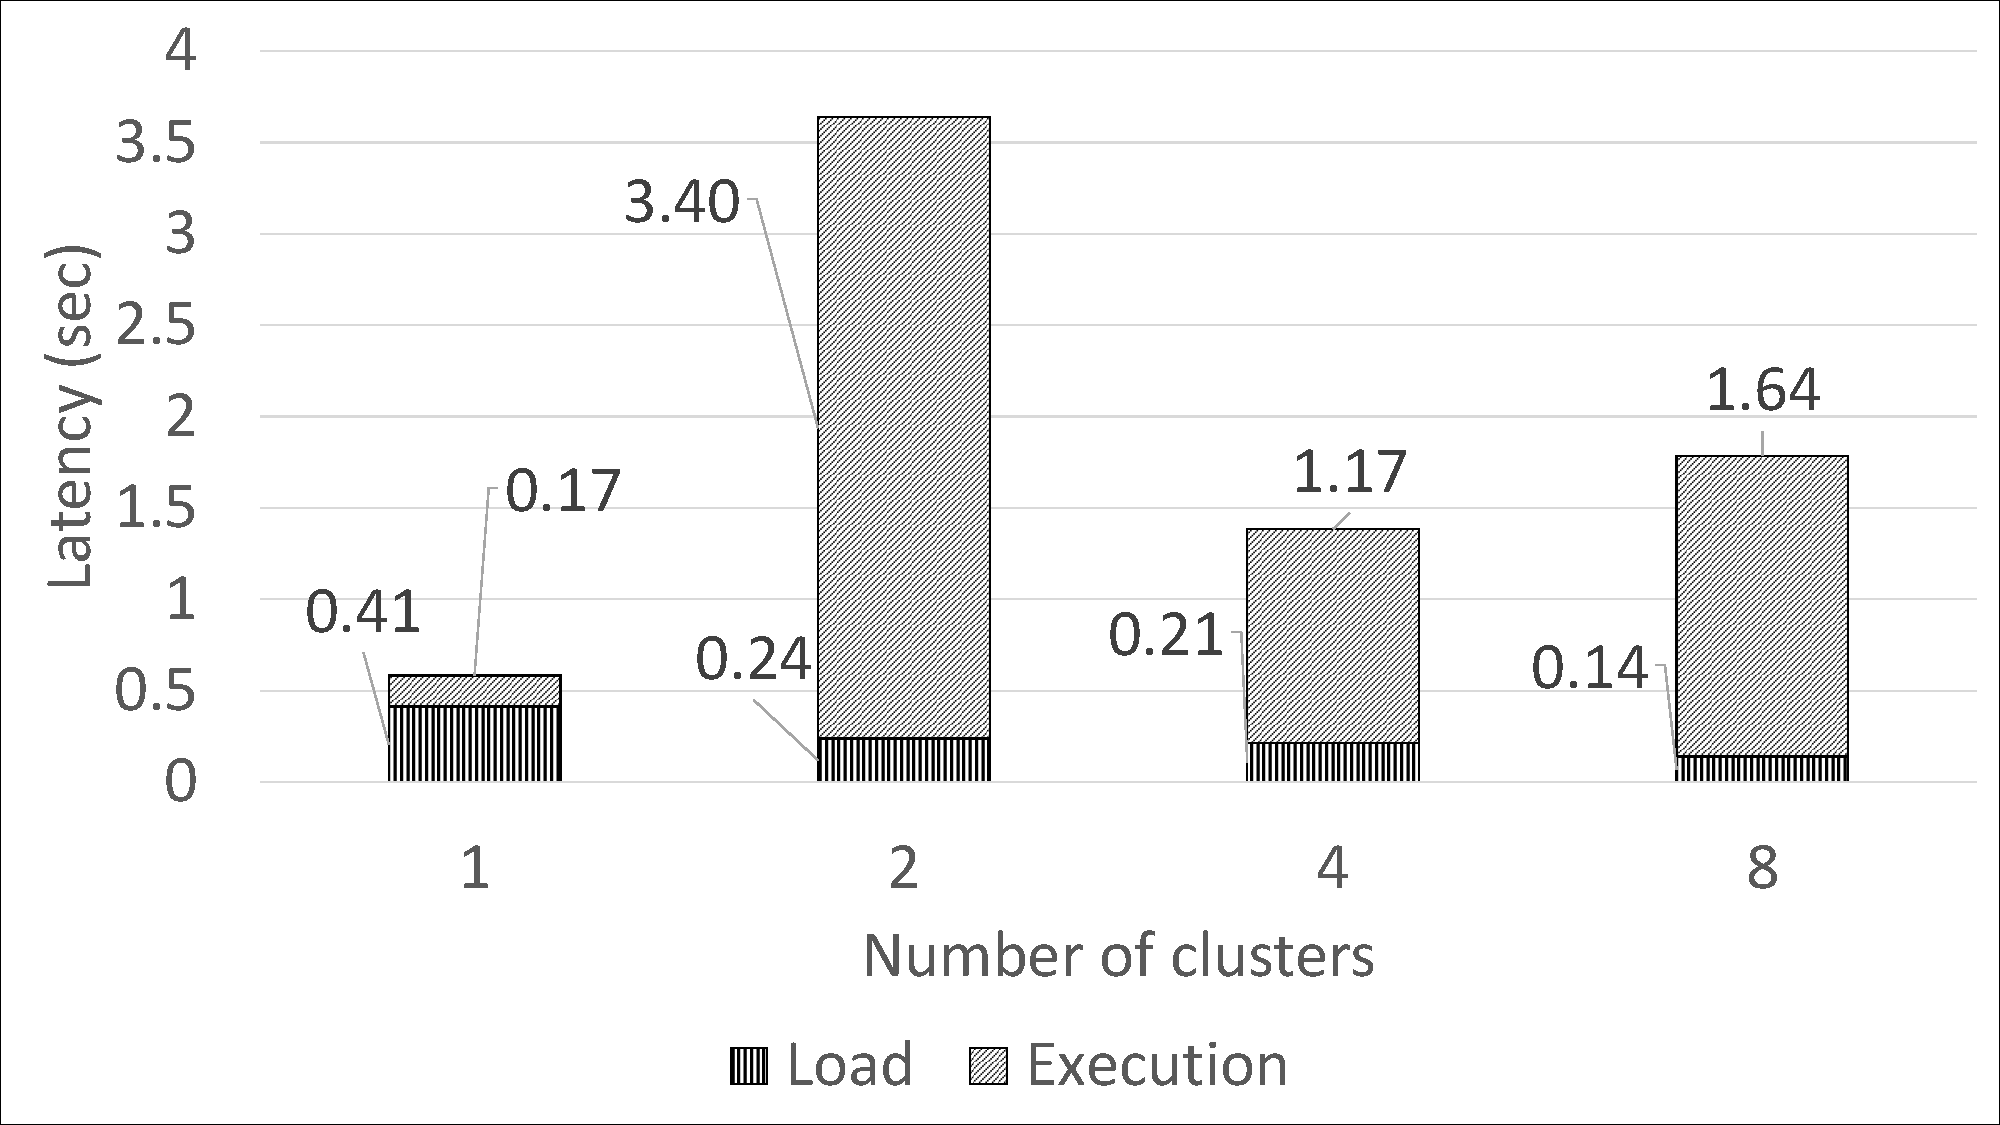
\includegraphics[width=0.4\textwidth]{evaluation/agglomerative_latency.pdf}}
       \subfigure[Accuracy (K-means)\label{fig:kmeans_impr_accuracy}]
       {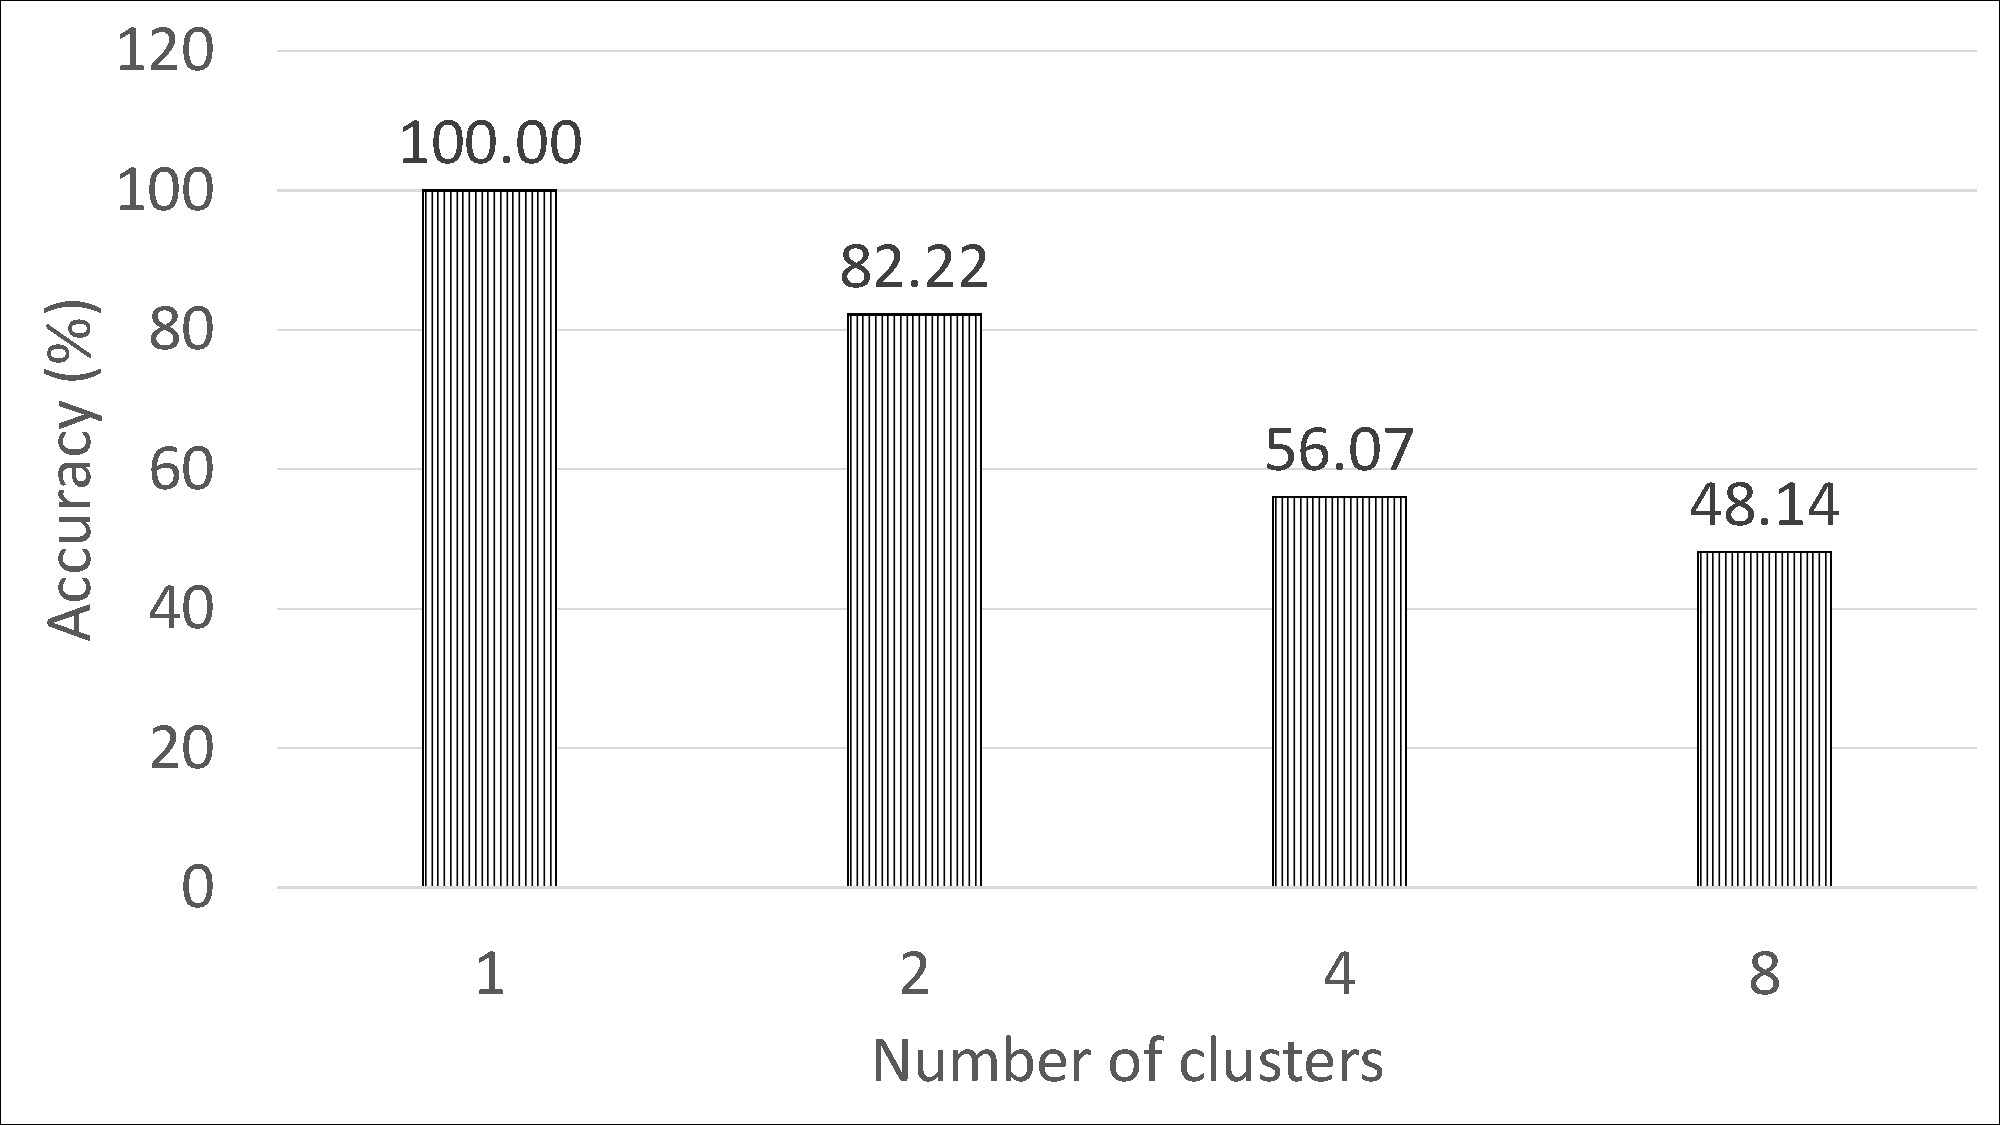
\includegraphics[width=0.4\textwidth]{evaluation/kmeans_accuracy.pdf}}
       \subfigure[Accuracy (Agglomerative)\label{fig:agglomerative_impr_accuracy}]
       {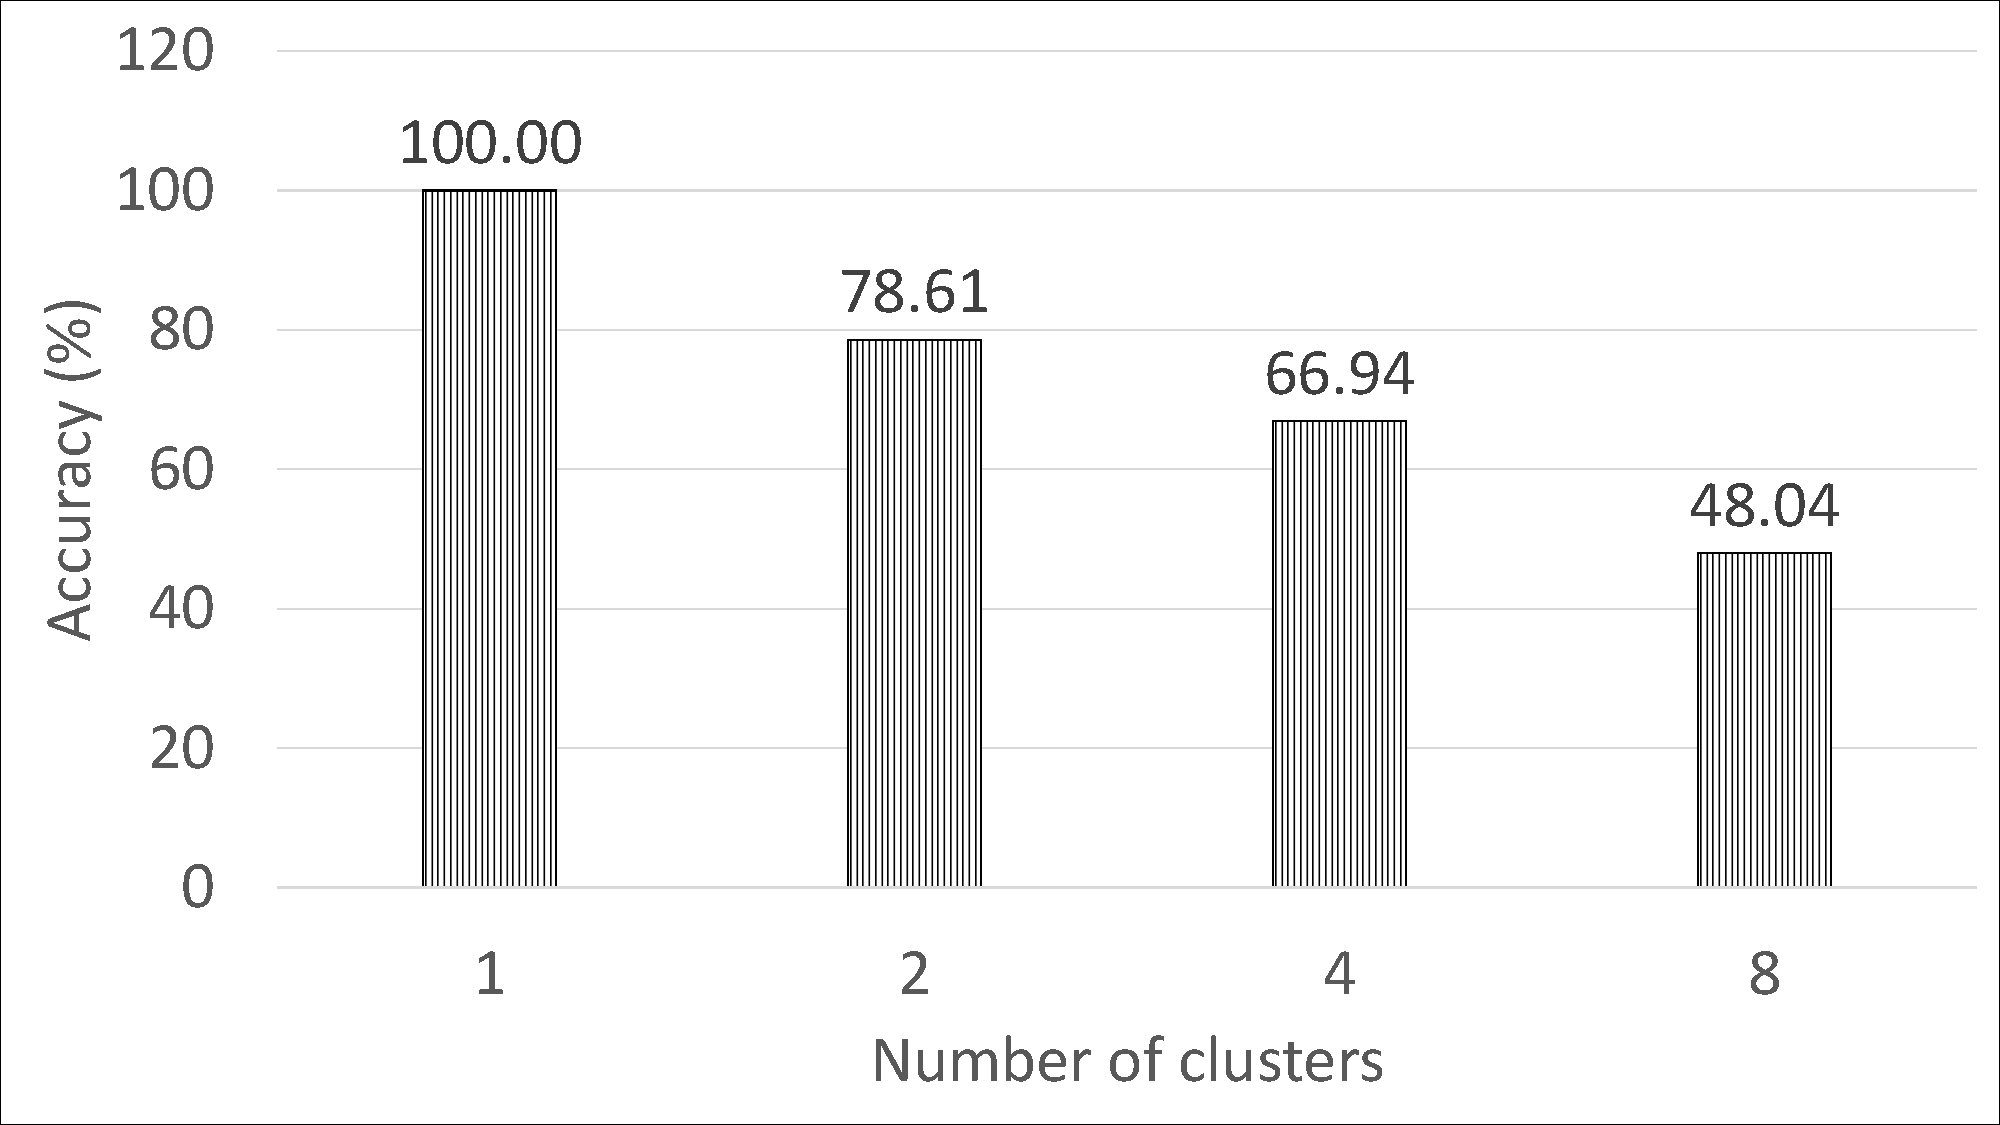
\includegraphics[width=0.4\textwidth]{evaluation/agglomerative_accuracy.pdf}}
       \vspace{-0.0pc}
       \caption{Improved latency breakdown and accuracy for distributed shortest path detection algorithm on data clustered using K-means and Agglomerative clustering}
       \label{fig:impr_eval}
    \end{center}
  \vspace{-1.0pc}
\end{figure*}

\subsubsection{Latency Evaluation}
\label{sec:latency_eval}
We measure the latency for both K-means and Agglomerative clustering in the initial implementation and the improved imeplementation.
In case of detecting the shortest path using the data clustered through K-means clustering, we observe that most of the latency
overhead occur in the user space. As shown in \figurename~\ref{fig:kmeans_init_latency} for K-means, with increasing number of clusters,
the time measured for the user space application execution increased drastically from 2.53 seconds for 1 cluster to 57.06 seconds
for 8 clusters, while the kernel space latency does not increase that much, i.e., from 1.82 seconds for 1 cluster to 10.08 seconds for 8 clusters.
Even though latency improvement was expected due to incorporating additional HPC resources, the high deependency among each
clusters for the geographic map data made difficult for the application and kernel to resolve the dependency among parallel units
of data. On the other hand, the data clustered using Agglomerative clustering technique behaved much better than that clustered using K-means.
For instance, as shown in \figurename~\ref{fig:agglomerative_init_accuracy}, the user space latency increased less steeply, i.e.,
from 2.93 seconds for 1 cluster to 11.049 seconds for 8 clusters. This is about 90\% improvement for 4 clusters and about 80\% improvement for
8 clusters. The kernel space latency also improved a lot for Agglomerative clustering. It was only 1.924 seconds for 1 cluster, stayed
almost the same for 2 and 4 clusters, and increased slightly to 3.1 seconds for 8 clusters.

Although we observed improvement by using data clustered by Agglomerative clustering technique, the latency measures were not only
higher than what we anticipated while planning the project, but also it was taking a lot of time in the user space. This means
there are problems in the algorithm implementation. After some profiling, we pinpointed the code snippet that was
creating performance bottleneck, i.e., the all source gateways to all destination gateways shortest path determination.
After this improvement, we ignored the kernel space latency and only focused on the user space latency. We further break the
latency down to data loading time from preprocessed pickle files and actual execution time of the distributed algorithm.
As shown in \figurename~\ref{fig:kmeans_impr_latency}, for K-means, the latency increased from 0.12 seconds for 1 cluster,
increased to 5.24 seconds for 4 clusters, and decreased to 2.28 seconds for 8 clusters. We observe about 56\% improvement
from cluster 4 to 8. On the other hand, for Agglomerative clustering, as stated in \figurename~\ref{fig:agglomerative_impr_latency},
the latency for the algorithm execution increased from 0.17 seconds for the whole graph to 3.40 seconds for 2 clusters.
Later, it had about 65\% decrement to 1.17 seconds for 4 clusters and increased a little to 1.64 seconds for 8 clusters.
For choosing Agglomerative clustering over K-means clustering, we can achieve about 78\% improvement in latency in this improved case.
For data loading time, it decreased slightly from 0.42 seconds for whole graph to 0.13 seconds for 8 clusters for K-means,
and 0.41 seconds for whole graph and 0.14 seconds for 8 clusters for Agglomerative clustering. This is obvious, because
with increased cluster numbers, we assign more HPC resources and each computing client have to read less amount of data.

\subsubsection{Accuracy Measurement}
\label{sec:accuracy_eval}
In the accuracy measurement, we compare the paths reported by the algorithm using the data from each clustering configuration
for different cluster numbers with the same path found from running the algorithm in 1 cluster or the whole graph.
We know that the whole graph contains all the connectivity and the path detected from whole graph is the ideal case scenario.
For calculating the output accuracy, we followed the equation below.
\[accuracy = n_c / n_i\]
where, $n_c$ = number of common nodes in ideal and given path, and $n_i$ = number of nodes in the ideal path.

As shown in \figurename~\ref{fig:kmeans_init_accuracy}, for K-means clustering, the accuracy is 100\% for 2 clusters,
but it drastically drops to 28.12\% for 4 clusters and got a little better to 55.45\% for 8 clusters.
On the contrary, for Agglomerative clustering, as depicted in \figurename~\ref{fig:agglomerative_init_accuracy},
we observed better accuracy trend than that for K-means clustered data, though it is quite less than what is expected
in general. For number of clusters more than 1, the accuracy stays in the range to 52.98\% to 59.6\%.

We measured the accuracy again after the code optimization discussed in Sec.~\ref{sec:latency_eval}.
This latency improvement impacted the accuracy a little, but in general it reported better accuracy
trend for different clustering configurations.
For instance, as shown in \figurename~\ref{fig:kmeans_impr_accuracy} for K-means clustering, the accuracy
dropped from 82.22\% to 48.14\% for 2 and 8 clusters respectively. For Agglomerative clustering, as depicted
in \figurename~\ref{fig:agglomerative_impr_accuracy}, it decreased from 78.61\% to 48.04\% for 2 and 8 clusters
respectively. Only for 4 clusters, data clustered by Agglomerative technique reports better accuracy (66.94\%) than
that (56.07\%) found by K-means data. In general, K-means and Agglomerative clustering demonstrate similar accuracy
trends.

\paragraph{Remarks}
The accuracy of the algorithm decreases with increasing number of clusters, because incorporating the clustered data
loses the inter-cluster connectivity information of the entire graph while running the algorithm in the
clustered data unit assigned to each process per client. Finally, after determining the final path by reducing
all the connectivity information via the gateway graph, we end up not finding the optimal solution. Nevertheless,
we get a suboptimal solution that represents a path from source node to the destination node.
